\documentclass{article}
\usepackage[margin=1in]{geometry}
\usepackage{amsmath}
\usepackage{amsfonts}
\usepackage{graphicx}
\input{sym}

\title{ECE 417 Midterm 1}
\date{Feb 18th, 2021}
\author{Vikas Dhiman}

\newtheorem{prob}{Problem}
\newif\ifsol
\solfalse

\begin{document}
\maketitle

\begin{tabular}{p{0.5\linewidth}p{0.5\linewidth}}
  (1) Student name:& Student email: \\
\end{tabular}

\subsubsection*{About the exam}
\begin{enumerate}
  \item There are total 5 problems. You must attempt all 5. 
  \item Maximum marks: 50 (70 with bonus).
  \item Maximum time allotted:  50 min
  \item Calculators are allowed.
  \item One US Letter size or A4 size cheat sheet (both-sides) is allowed.
\end{enumerate}

\begin{prob}
  What are the two criteria for a $3 \times 3$ matrix $A$ to be a valid rotation matrix?
  (5 min, 5 marks)
\end{prob}
\newpage

\begin{prob}
  For Fig~\ref{fig:rot-2D}, write the rotation matrix $R(\theta)$ that converts
  between coordinates of point from red coordinate frame $\bfp_c$ to green
  coordinate frame $\bfp_w$ such that $\bfp_w = R(\theta) \bfp_c$. (Optional
  part) Test your
  formula if it looks correct for $\theta  = -30^\circ$, $\bfp_c
  = \begin{bmatrix} 1 \\ 3 \end{bmatrix}$.
  (5 min, 5 marks)
\end{prob}

\begin{figure}
  \centering
  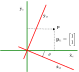
\includegraphics[width=0.5\linewidth]{media/rot-2D.pdf}
  \caption{Rotation between red frame and green coordinate frame.}
  \label{fig:rot-2D}
\end{figure}

\newpage

\begin{prob}
  In Figure~\ref{fig:Rodrigues-formula}, we are rotating point $\bfv$ around
  axis unit-vector $\hat{\bfk}$ by an angle $\theta$. $\bfv_{\perp}$ lies in the plane of $\bfv$
  and $\hat{\bfk}$ and is orthogonal (perpendicular) to $\bfk$. $\bfw$ is
  perpendicular to the plane of $\bfv$ and $\hat{\bfk}$. First, write the
  unit-vector $\hat{\bfw}$ in terms of $\bfv$ and $\hat{\bfk}$.
  Then write unit-vector $\hat{\bfv}_\perp$ in terms of $\bfv$ and $\hat{\bfk}$.
  (10 min, 10 marks)
\end{prob}
\begin{figure}
  \centering
  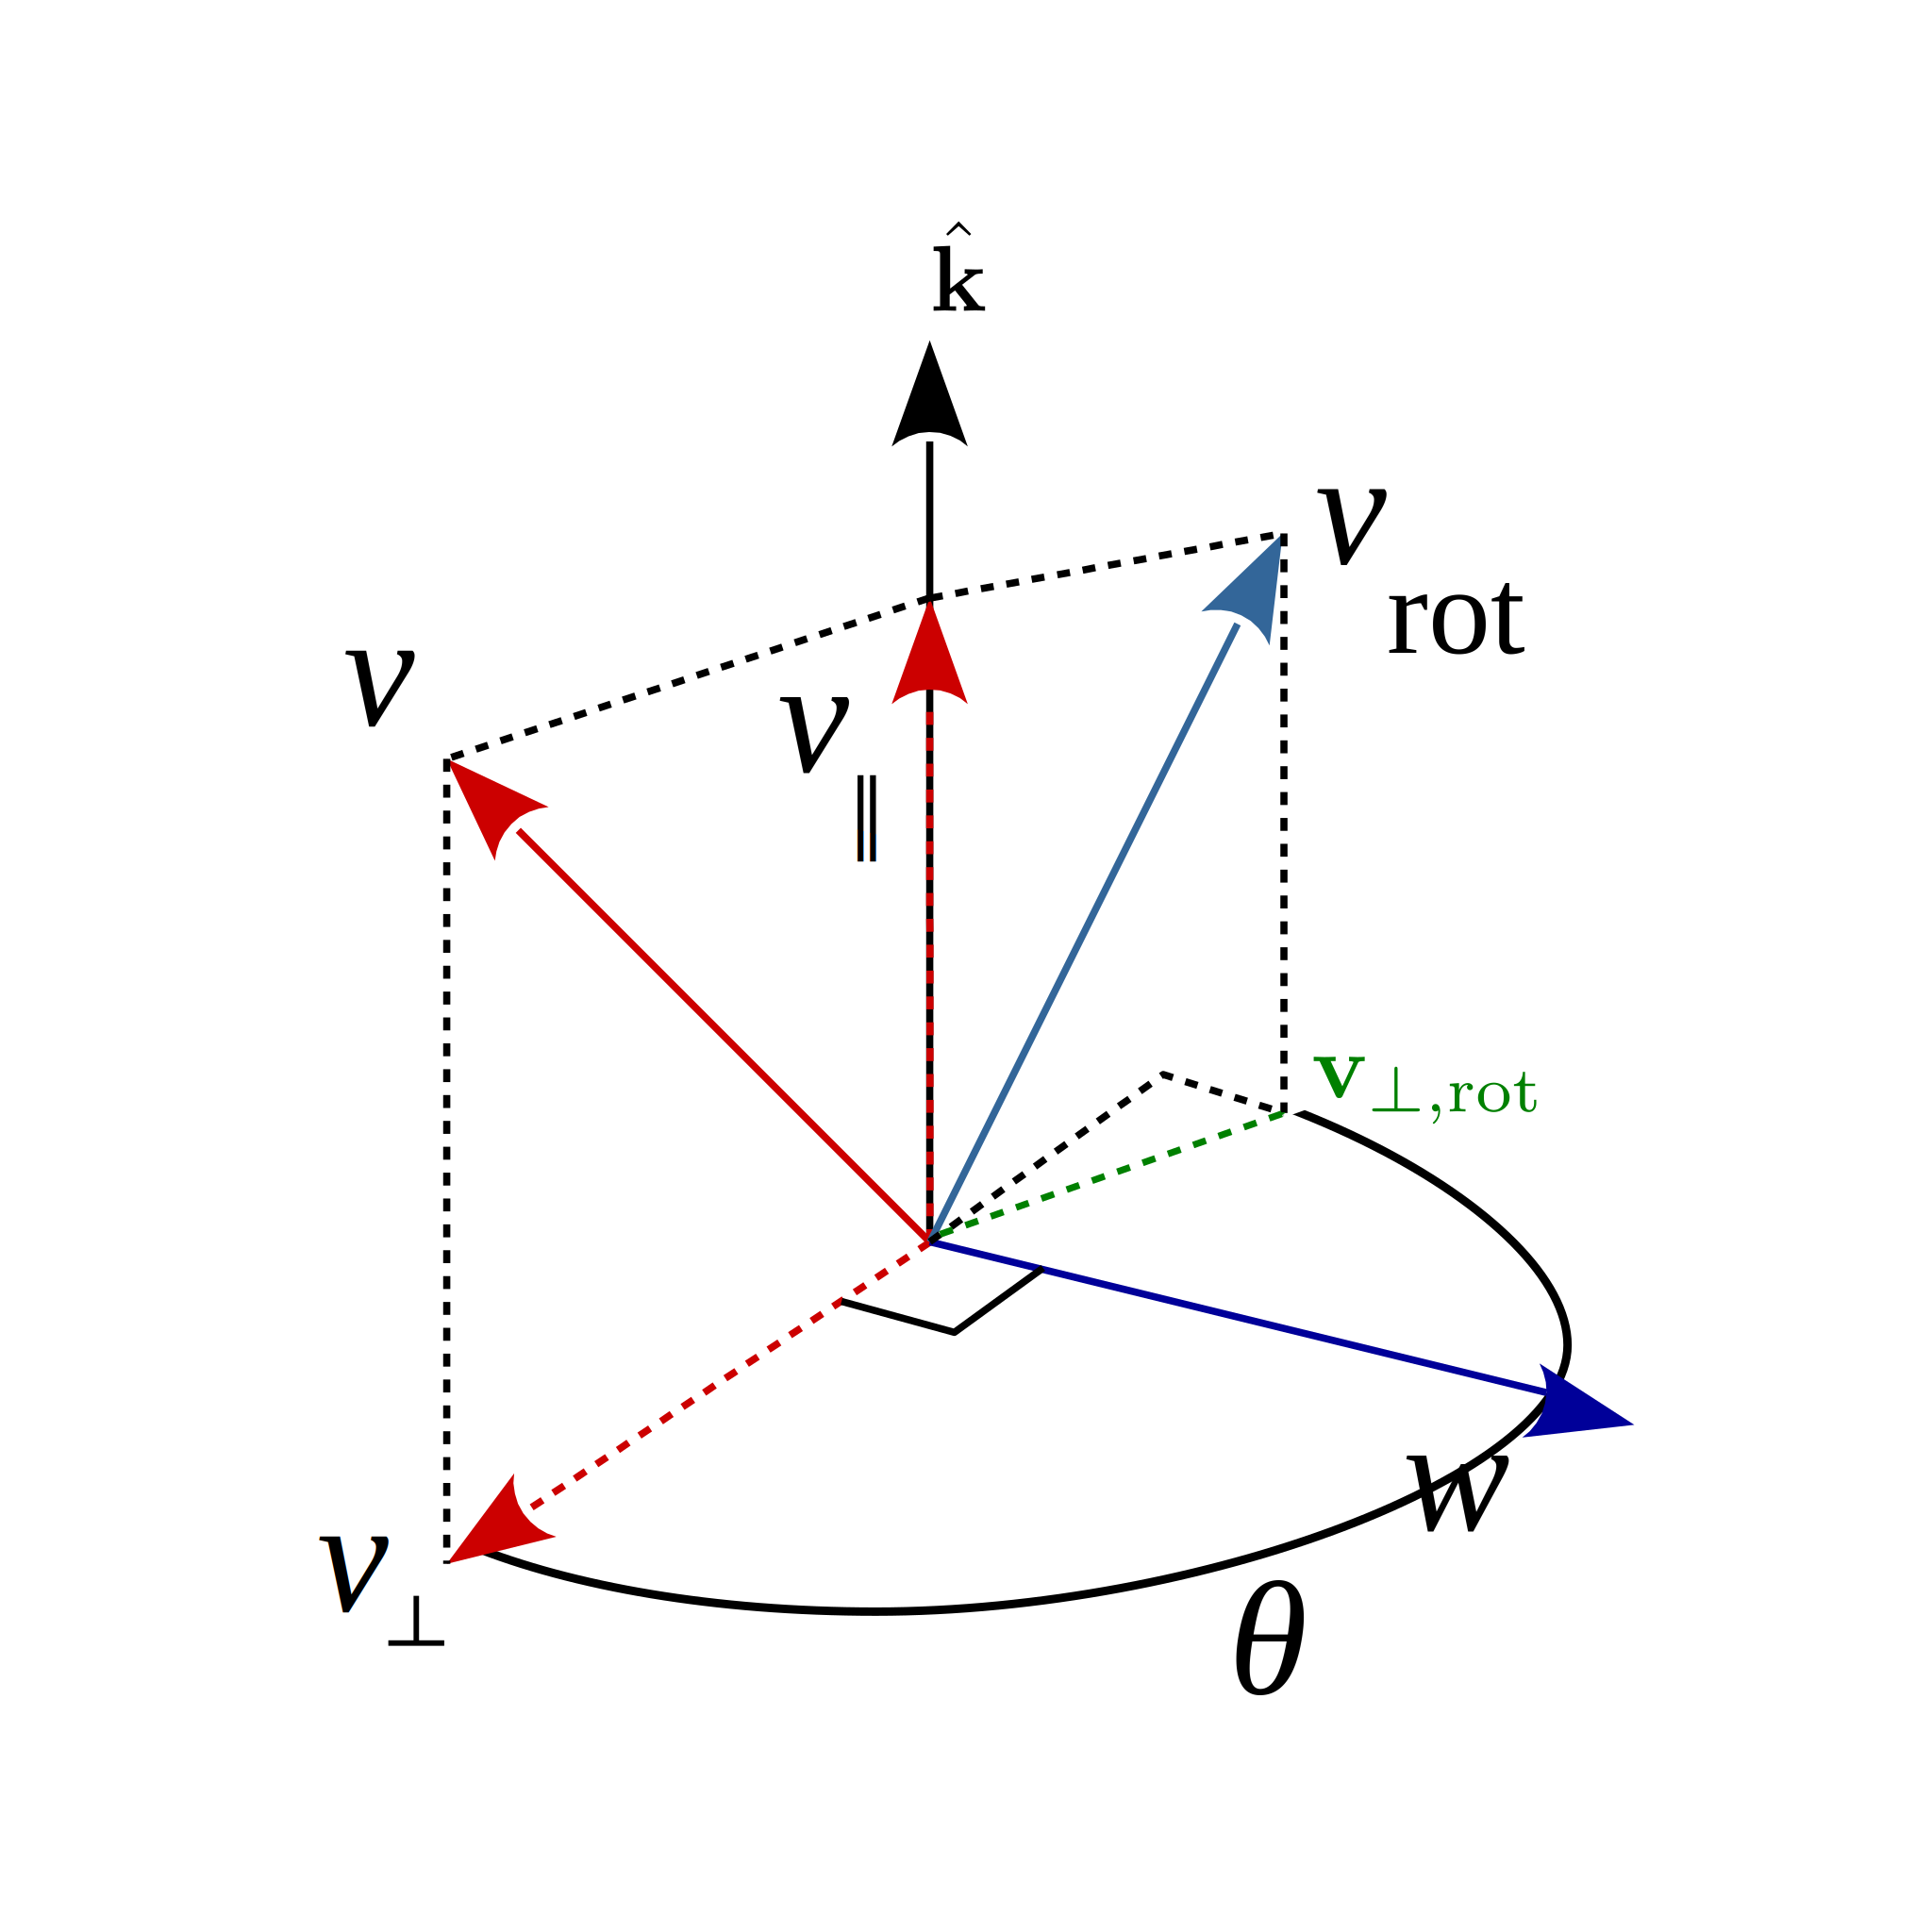
\includegraphics[width=0.5\linewidth]{media/Rodrigues-formula.pdf}
  \caption{Rotation of point $\bfv$ around axis $\bfk$ by angle $\theta$}
  \label{fig:Rodrigues-formula}
\end{figure}

\newpage
\begin{prob}
  Using the fact that at minima (or maxima) of a differentiable function
  $f(\bfx)$, $\nabla_\bfx f(\bfx) = 0$, find the minima of the following
  function,
  \begin{align}
    f(\bfx) = (\bfx - \bfp)^\top A^\top A (\bfx-\bfp) + 2 \bfb^\top \bfx + c,
  \end{align}
  where $\bfx \in \bbR^n$, $\bfp \in \bbR^n$, $\bfb \in \bbR^n$, $c \in \bbR$,
  $A \in \bbR^{m \times n}$. Assume $A^\top A$ to be invertible.
  (10 min, 10 marks)
\end{prob}

\newpage

\begin{prob}
  In figure~\ref{fig:image-road-triangulation} find the 3D position of mercedes logo
  in the World coordinate frame, in terms of $h$ (the height of the camera),
  image-coordinates of the mercedes logo $\bfu$, camera matrix $K$, and $h_2$
  the height of logo from the road. The Camera mounted directly on top of the
world frame. The road is a perfect plane and the pothole lies on the road plane
(Equation of plane $Z_w = 0$ in the world coordinate frame). You do not need to
substitute in the values, providing a formula or pseudo-code for computing the
pothole coordinates is enough. (20 min, 20 marks, Bonus marks: 20)
\end{prob}

\begin{figure}
  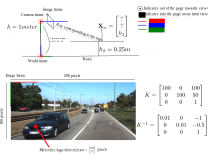
\includegraphics[width=\linewidth]{media/image-road-triangulation.pdf}
  \caption{Image road triangulation}
  \label{fig:image-road-triangulation}
\end{figure}


\end{document}
